\documentclass{beamer}
\usepackage{geometry}
\usepackage[english]{babel}
\usepackage[utf8]{inputenc}
\usepackage{amsmath}
\usepackage{amsfonts}
\usepackage{amssymb}
\usepackage{tikz}
\usetikzlibrary{quotes, angles}
\usepackage{graphicx}
\usepackage{multicol}

%\usepackage{pgfplots}
%\pgfplotsset{width=10cm,compat=1.9}
%\usepackage{pgfplotstable}

\setlength{\headheight}{26pt}%doesn't seem to fix warning

\usepackage{fancyhdr}
\pagestyle{fancy}
\fancyhf{}

%\rhead{\small{3 September 2019}}
\lhead{\small{BECA / Dr. Huson / Geometry Unit 1 Quiz}}

\renewcommand{\headrulewidth}{0pt}

\title{Mathematics Class Slides}
\subtitle{Bronx Early College Academy}
\author{Christopher J. Huson PhD}
\date{7-15 October 2020}

\begin{document}
%\frame{\titlepage}
\section[Outline]{}
%\frame{\tableofcontents}


\frame
{
  \frametitle{\\Unit 1 Quiz: Introduction to Geometry}
  \framesubtitle{What do you know? What can you do?  \hfill \alert{Thursday, Friday October 15, 16}} 
    Demonstrate mastery of the following standards:
    \begin{enumerate}
      \item Applying vocabulary and notation, diagrams
      \item Applying the Segment Addition Postulate, length
      \item Quantitative operations on the number line
    \end{enumerate}

}

\frame
  {
    \frametitle{1) Diagrams and notation}
    Identify the objects shown in the diagram. Type your answer on the blank line and be sure to use small or capital letters correctly.
    \begin{enumerate} \vspace{0.5cm}
      \item The intersection of the two lines:  \rule{3cm}{0.15mm} \bigskip
      \item The name of the plane:  \rule{3cm}{0.15mm} \bigskip
      \end{enumerate}
      \begin{center}
        \begin{tikzpicture}
        \draw [thick](0,0) node[above right]{$\ n$} --(6,0)--(8,4)--(2,4)--(0,0);
        \draw [<->, thick] (2, 1.4)--(6,3);
        \draw [fill] (4, 3.5) circle [radius=0.05] node[below]{$J$};
        %\draw [fill] (2, 1.4) circle [radius=0.05] node[below]{$B$};
        \draw [fill] (3.5,2) circle [radius=0.05] node[below]{$K \ $};
        \draw [fill] (5,2.6) circle [radius=0.05] node[below]{$L$};
        \draw [<->, thick] (2,3.5)--(5.25,.25);
        \draw [fill] (5,0.5) circle [radius=0.05] node[above right]{$M \ $};
      \end{tikzpicture}
    \end{center}
  }

  \frame
  {
    \frametitle{2) Diagrams and notation}
      What is shown in the diagram? Mark all that apply.
      \begin{enumerate}
        \item A rectangle
        \item An equilateral triangle
        \item An isosceles triangle
        \item A triangle that is neither isosceles nor equilateral
      \end{enumerate}
      \begin{center}
        \begin{tikzpicture}[scale=0.5]
          \draw [thick](0,0)--(4,0)--(2,6)--(0,0);
          \draw [fill] (0,0) circle [radius=0.05] node[below]{$A$};
          \draw [fill] (4,0) circle [radius=0.05] node[below]{$B$};
          \draw [fill] (2,6) circle [radius=0.05] node[right]{$C$};
          \draw [thick] (0.8,3.1)--(1.2,3); %tick mark
          \draw [thick] (2.8,3)--(3.2,3.1); %tick mark
        \end{tikzpicture}
      \end{center}
  }

  \frame
  {
    \frametitle{3) Diagrams and notation}
    Given the points $D$ and $E$, draw ray $\overrightarrow{DE}$.
    \vspace{1.5cm}
    \begin{center}
      \begin{tikzpicture}
      \draw [fill] (0,2) circle [radius=0.05] node[right]{$D$};
      \draw [fill] (0,0) circle [radius=0.05] node[right]{$E$};
    \end{tikzpicture}
    \end{center} \vspace{1cm}
  }

  \frame
  {
    \frametitle{4)  Diagrams and notation}
      Given isosceles $\triangle XYZ$ with $\overline{XY} \cong \overline{XZ}$.\\[0.5cm]
      On the diagram mark the congruent line segments with tick marks. \vspace{1cm}
      \begin{center}
      \begin{tikzpicture}[scale=0.3]
        \draw [thick](0,0)--(9,0)--(4,8)--(0,0);
        \draw [fill] (0,0) circle [radius=0.05] node[below]{$X$};
        \draw [fill] (9,0) circle [radius=0.05] node[below]{$Y$};
        \draw [fill] (4,8) circle [radius=0.05] node[above right]{$Z$};
      \end{tikzpicture}
      \end{center}
  }

  \frame
  {
    \frametitle{5) Applying the segment addition postulate}
      Given $\overline{JKL}$, $JK=8.4$, and $KL=2.7$. Find ${JL}$.\\[0.5cm]
      Show your work by marking the diagram and writing an equation.\\[2cm]
        \begin{tikzpicture}
          \draw [-, thick] (0,0)--(7,0);
          \draw [fill] (0,0) circle [radius=0.05] node[below]{$J$};
          \draw [fill] (5,0) circle [radius=0.05] node[below]{$K$};
          \draw [fill] (7,0) circle [radius=0.05] node[below]{$L$};
        \end{tikzpicture} \vspace{4cm}
  }

  \frame
  {
    \frametitle{6) Applying the segment addition postulate}
    Given $\overline{PQR}$, $PQ=2x+2$, $QR=8$, $PR=20$. Find ${x}$.
    \begin{center}
       \begin{tikzpicture}
        \draw [-, thick] (0,0)--(7,0);
        \draw [fill] (0,0) circle [radius=0.05] node[below]{$P$};
        \draw [fill] (4,0) circle [radius=0.05] node[below]{$Q$};
        \draw [fill] (7,0) circle [radius=0.05] node[below]{$R$};
        \node at (2,0) [above]{$2x+2$};
        \node at (5.5,0) [above]{$8$};
        \draw [<->, dashed] (0,-0.7)--(7,-0.7);
        \node at (3.5,-0.7) [below]{$20$};
      \end{tikzpicture}
    \end{center}
  \begin{enumerate}
      \item Write down an equation to represent the situation. \vspace{0.5cm}
      \item Solve for $x$. \vspace{1.5cm}
      \item Check your answer. \vspace{2cm}
    \end{enumerate}
  }

  \frame
  {
    \frametitle{7) Applying the segment addition postulate}
      Find the perimeter of the isosceles $\triangle FGH$, given $\overline{FH} \cong \overline{GH}$, $FG=5$, and $FH=8 \frac{1}{4}$\\[0.25cm]
      Show your work with an equation for full credit.\\[0.5cm]
        \begin{tikzpicture}[scale=0.5]
          \draw [thick](0,0)--(4,0)--(2,6)--(0,0);
          \draw [fill] (0,0) circle [radius=0.05] node[below left]{$F$};
          \draw [fill] (4,0) circle [radius=0.05] node[below right]{$G$};
          \draw [fill] (2,6) circle [radius=0.05] node[above right]{$H$};
          \draw [thick] (0.8,3.1)--(1.2,3); %tick mark
          \draw [thick] (2.8,3)--(3.2,3.1); %tick mark
          \node at (2,0) [below]{$5$};
          \node at (0.8,3.4) [left]{$8 \frac{1}{4}$};
        \end{tikzpicture} \vspace{1cm}
  }

  \frame
  {
    \frametitle{8) Applying the segment addition postulate}
      The midpoint $M$ bisects the line segment $\overline{AB}$ and $AB=12$.
      \begin{enumerate}
        \item Mark and label the approximate location of $M$.
        \item Find ${AM}$. State an equation for full credit.
      \end{enumerate} \vspace{1cm} 
      \begin{center}
        \begin{tikzpicture}
          \draw [-, thick] (0,0)--(6,0);
          \draw [fill] (0,0) circle [radius=0.05] node[below]{$A$};
          \draw [fill] (6,0) circle [radius=0.05] node[below]{$B$};
        \end{tikzpicture} 
      \end{center} \vspace{3cm} 
  }

  \frame
  {
    \frametitle{9) Finding lengths on the number line}
    Given $\overline{MN}$ with $M(1)$ and $N(5)$. \\[1.5cm]
      \begin{tikzpicture}
        \draw [<->] (-3.5,0)--(6.5,0);
        %\draw [-, thick] (1,0)--(4.5,0);
        \foreach \x in {-3,...,6} %2 leading for diff!=1
          \draw[shift={(\x,0)},color=black] (0pt,-3pt) -- (0pt,3pt) node[below=5pt]  {$\x$};
          %\draw [fill] (1,0) circle [radius=0.05] node[above] {$M$};
          %\draw [fill] (4.5,0) circle [radius=0.05] node[above] {$N$};
      \end{tikzpicture}
      \begin{enumerate}
        \item Mark and label the points and segment on the number line.
        \item Find the length ${MN}$. Show your work as an equation.
        \item Check your work by counting the distance. Leave marks to show your work.
      \end{enumerate} \vspace{2cm}  
  }

  \frame
  {
    \frametitle{10) Finding lengths on the number line}
    Given $G(-1)$ and $H(2.7)$, as shown on the number line. \\[0.25cm]
    Find the length of the line segment $\overline{GH}$. State an equation for full credit. \\
      \begin{tikzpicture}
        \draw [<->] (-4.5,0)--(4.5,0);
        \draw [-, thick] (-1,0)--(2.7,0);
        \foreach \x in {-4,...,4} %2 leading for diff!=1
          \draw[shift={(\x,0)},color=black] (0pt,-3pt) -- (0pt,3pt) node[below=5pt]  {$\x$};
          \draw [fill] (-1,0) circle [radius=0.05] node[above] {$G$};
          \draw [fill] (2.7,0) circle [radius=0.05] node[above] {$H$};
      \end{tikzpicture}
      \vspace{4cm}  
  }

  \frame
  {
    \frametitle{11) Finding lengths on the number line}
    Given point $A(1)$ as shown below. Locate point, $B > 0$, on the number line such that ${AB}=4 \frac{1}{2}$. \\[1.5cm]
      \begin{tikzpicture}
        \draw [<->] (-2.5,0)--(6.5,0);
        %\draw [-, thick] (1,0)--(4.5,0);
        \foreach \x in {-2,...,6} %2 leading for diff!=1
          \draw[shift={(\x,0)},color=black] (0pt,-3pt) -- (0pt,3pt) node[below=5pt]  {$\x$};
          \draw [fill] (1,0) circle [radius=0.05] node[above] {$A$};
          %\draw [fill] (4.5,0) circle [radius=0.05] node[above] {$N$};
      \end{tikzpicture}
      \begin{enumerate}
        \item Mark and label $B$.
        \item State the value of $B$, writing an equation to support your work.
      \end{enumerate} \vspace{3cm}  
  }

  \frame
  {
    \frametitle{12) Finding lengths on the number line}
    Given $S(-1)$ and $T(5)$, as shown on the number line. \\[0.25cm]
    Mark and label the midpoint $M$ that bisects $\overline{ST}$. \\[0.5cm]
      \begin{tikzpicture}
        \draw [<->] (-3.5,0)--(6.5,0);
        \draw [-, thick] (-1,0)--(5,0);
        \foreach \x in {-3,...,6} %2 leading for diff!=1
          \draw[shift={(\x,0)},color=black] (0pt,-3pt) -- (0pt,3pt) node[below=5pt]  {$\x$};
          \draw [fill] (-1,0) circle [radius=0.05] node[above] {$S$};
          \draw [fill] (5,0) circle [radius=0.05] node[above] {$T$};
      \end{tikzpicture} \vspace{4cm}  
  }

  \frame
  {
    \frametitle{13) Applying the segment addition postulate (spicy)}
    Given $M$ is the midpoint of $\overline{AB}$, $AM=7x+10$, $MB=31$.
    \begin{enumerate}
      \item Mark the diagram with the values and tick marks
      \item Write an equation and solve for $x$
      \item Check your result
    \end{enumerate} \vspace{1cm}
      \begin{center}
        \begin{tikzpicture}
          \draw [fill] (0,0) circle [radius=0.05] node[below]{$A$};
          \draw [-, thick] (0,0)--(7,0);
          \draw [fill] (3.5,0) circle [radius=0.05] node[below]{$M$};
          \draw [fill] (7,0) circle [radius=0.05] node[below]{$B$};
          %\node at (1.7,0.5) [above]{$x+2$};
          %\node at (5.2,0.5) [above]{$11$};
          %\draw [<->, dashed] (0,-1)--(7,-1);
          %\node at (3.5,-1) [below]{$20$};
        \end{tikzpicture}
      \end{center} \vspace{4cm}
  }

  \frame
  {
    \frametitle{14) Applying the segment addition postulate (spicy)}
      Given equilateral $\triangle ABC$ having perimeter of 11. Find the length of side $\overline{AB}$, $x$, as a fraction (not a decimal).\vspace{1cm}
      \begin{center}
      \begin{tikzpicture}[scale=0.3]
        \draw [thick](0,0)--(9,0)--(4,8)--(0,0);
        \draw [fill] (0,0) circle [radius=0.05] node[below]{$A$};
        \draw [fill] (9,0) circle [radius=0.05] node[below]{$B$};
        \draw [fill] (4,8) circle [radius=0.05] node[above right]{$C$};
        \node at (4.5,0) [below]{$x$};
      \end{tikzpicture}
      \end{center}
  }

  \frame
  {
    \frametitle{15) Applying the segment addition postulate (spicy)}
      Given the points $S$ and $T$ trisect the line segment $\overline{RU}$, as shown below. If $SU=6$, find $RU$.\\[1cm]
      \begin{tikzpicture}[scale=0.75]
       \draw [-, thick] (0,0)--(9,0);
       \draw [fill] (0,0) circle [radius=0.05] node[below]{$R$};
       \draw [fill] (3,0) circle [radius=0.05] node[below]{$S$};
       \draw [fill] (6,0) circle [radius=0.05] node[below]{$T$};
       \draw [fill] (9,0) circle [radius=0.05] node[below]{$U$};
       %\node at (1.6,0.3) [above]{$x$};
       %\node at (4.6,0.3) [above]{$x$};
       %\node at (7.6,0.3) [above]{$x$};
       \draw [-, thick] (1.4,-0.2)--(1.4,0.2);
       \draw [-, thick] (1.55,-0.2)--(1.55,0.2);
       \draw [-, thick] (4.4,-0.2)--(4.4,0.2);
       \draw [-, thick] (4.55,-0.2)--(4.55,0.2);
       \draw [-, thick] (7.4,-0.2)--(7.4,0.2);
       \draw [-, thick] (7.55,-0.2)--(7.55,0.2);
       %\draw [<->, dashed] (0,-1.3)--(9,-1.3);
       %\node at (4.5,-1.3) [below]{$15$};
     \end{tikzpicture} \vspace{3cm}
  }

\end{document}